\pdfoutput=1

\begin{figure*}[!htb]
    \centering
        
    \begin{subfigure}[b]{0.48\textwidth}
        \centering
        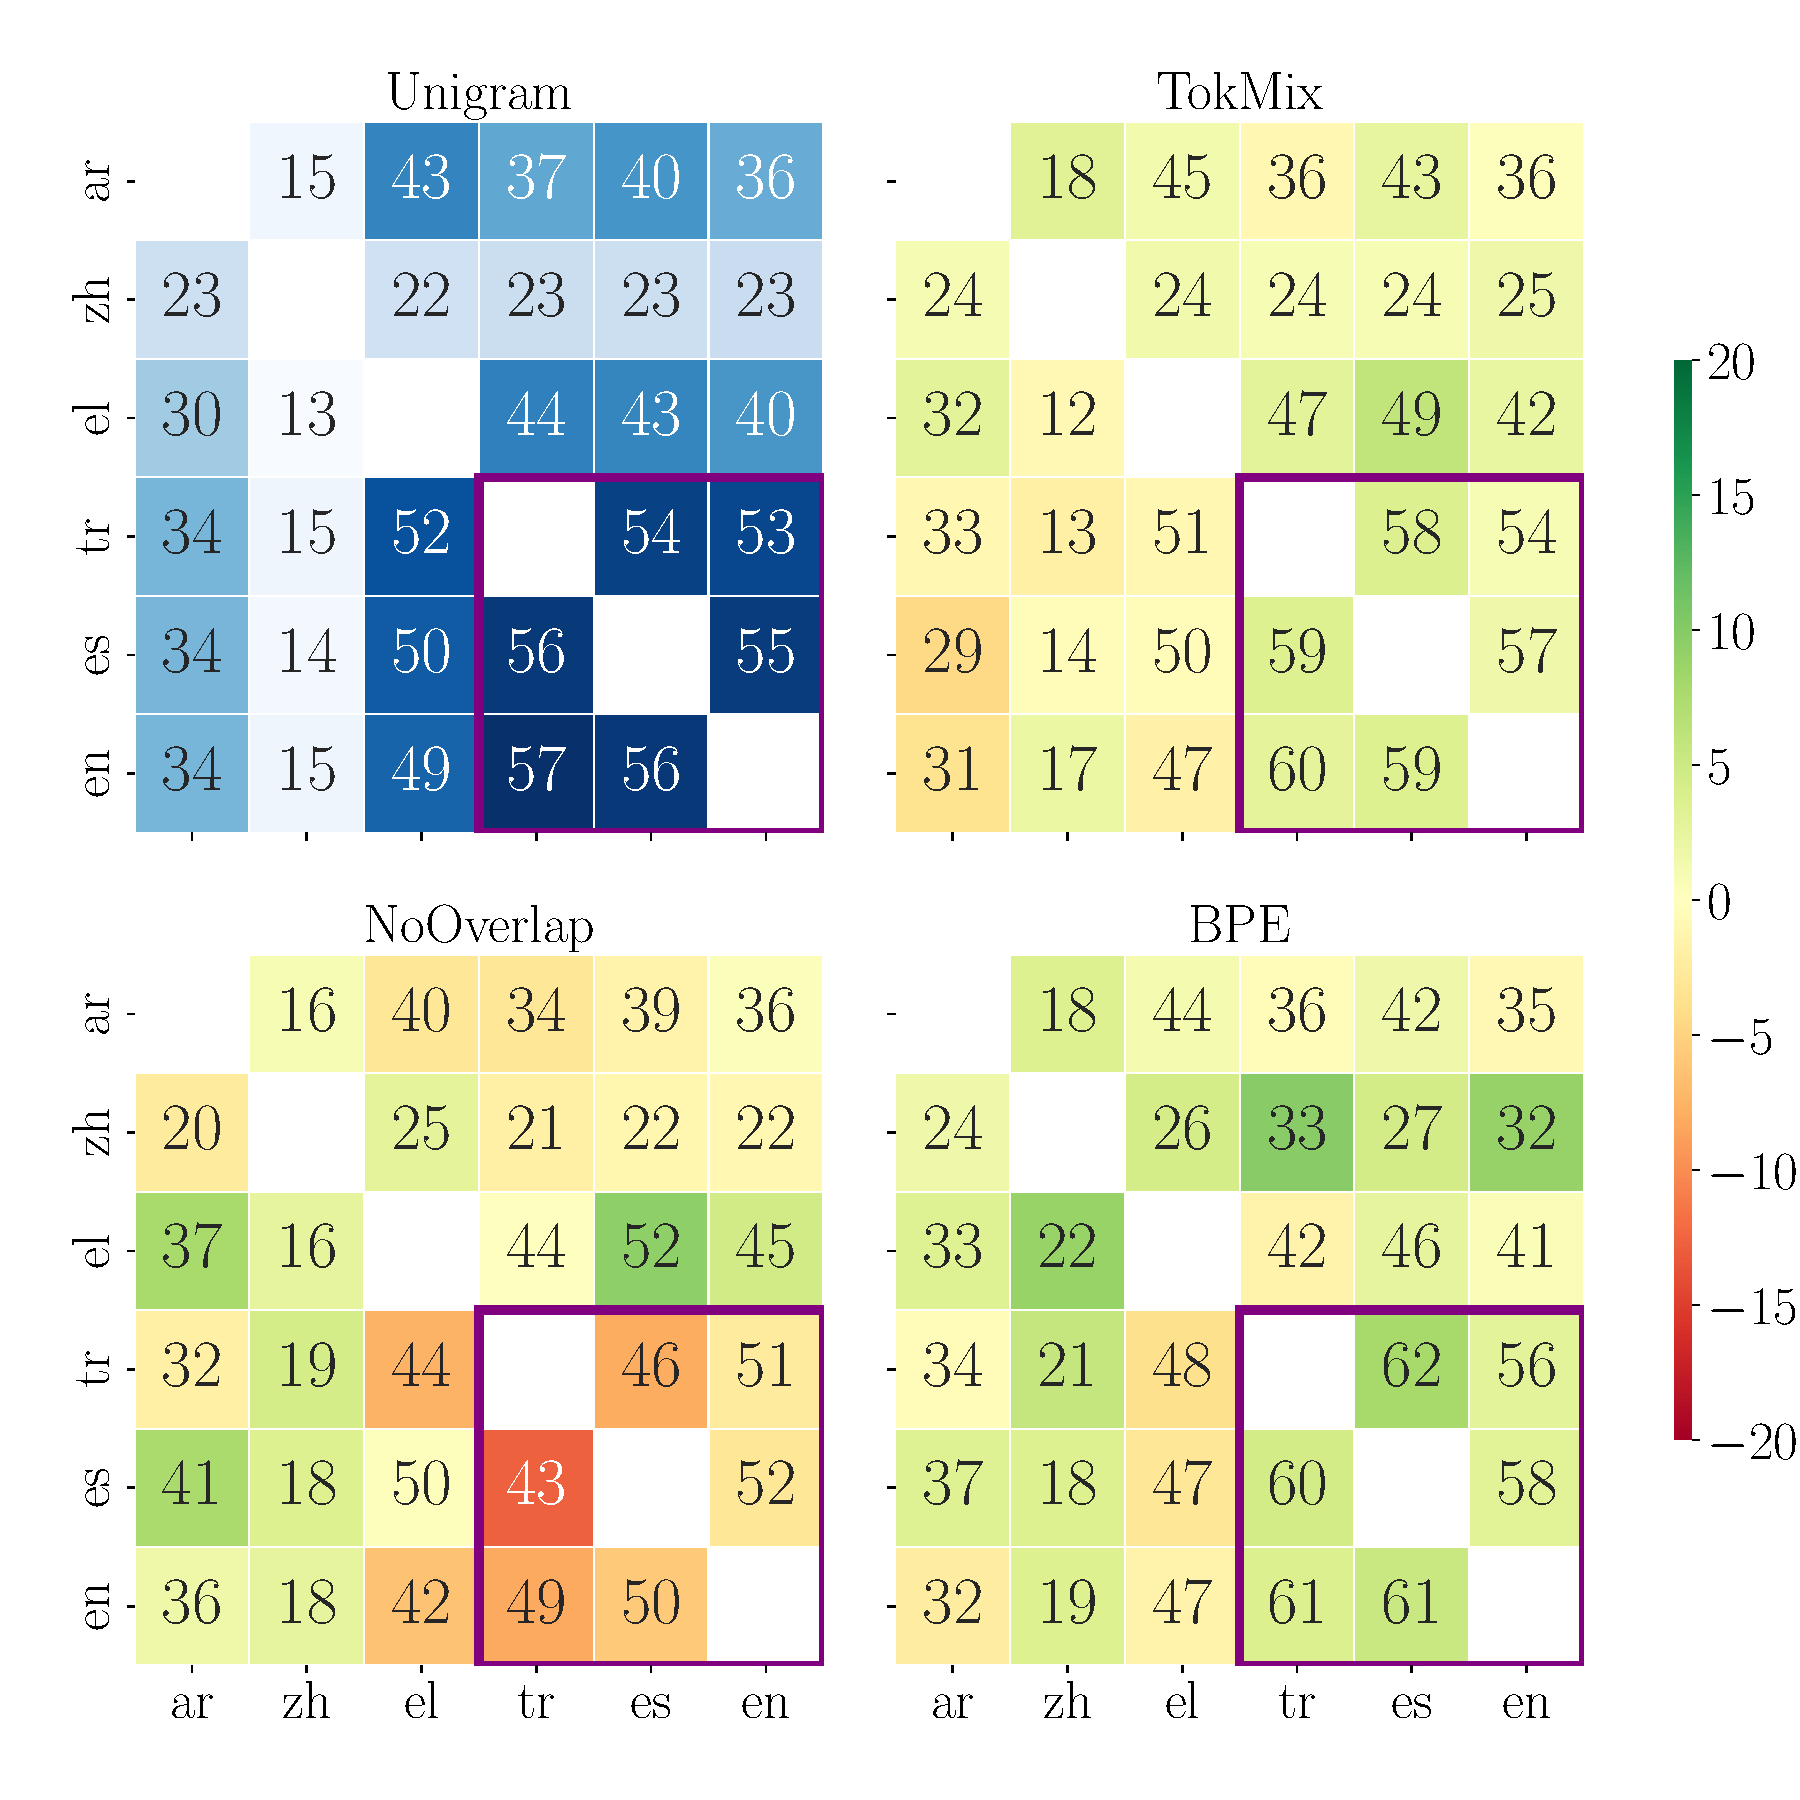
\includegraphics[width=\textwidth]{figures/NER_F1_transfer_.pdf}
        \caption{NER (F1)}
        \label{fig:ner_transfer}
    \end{subfigure}
    \hfill
    \begin{subfigure}[b]{0.48\textwidth}
        \centering
        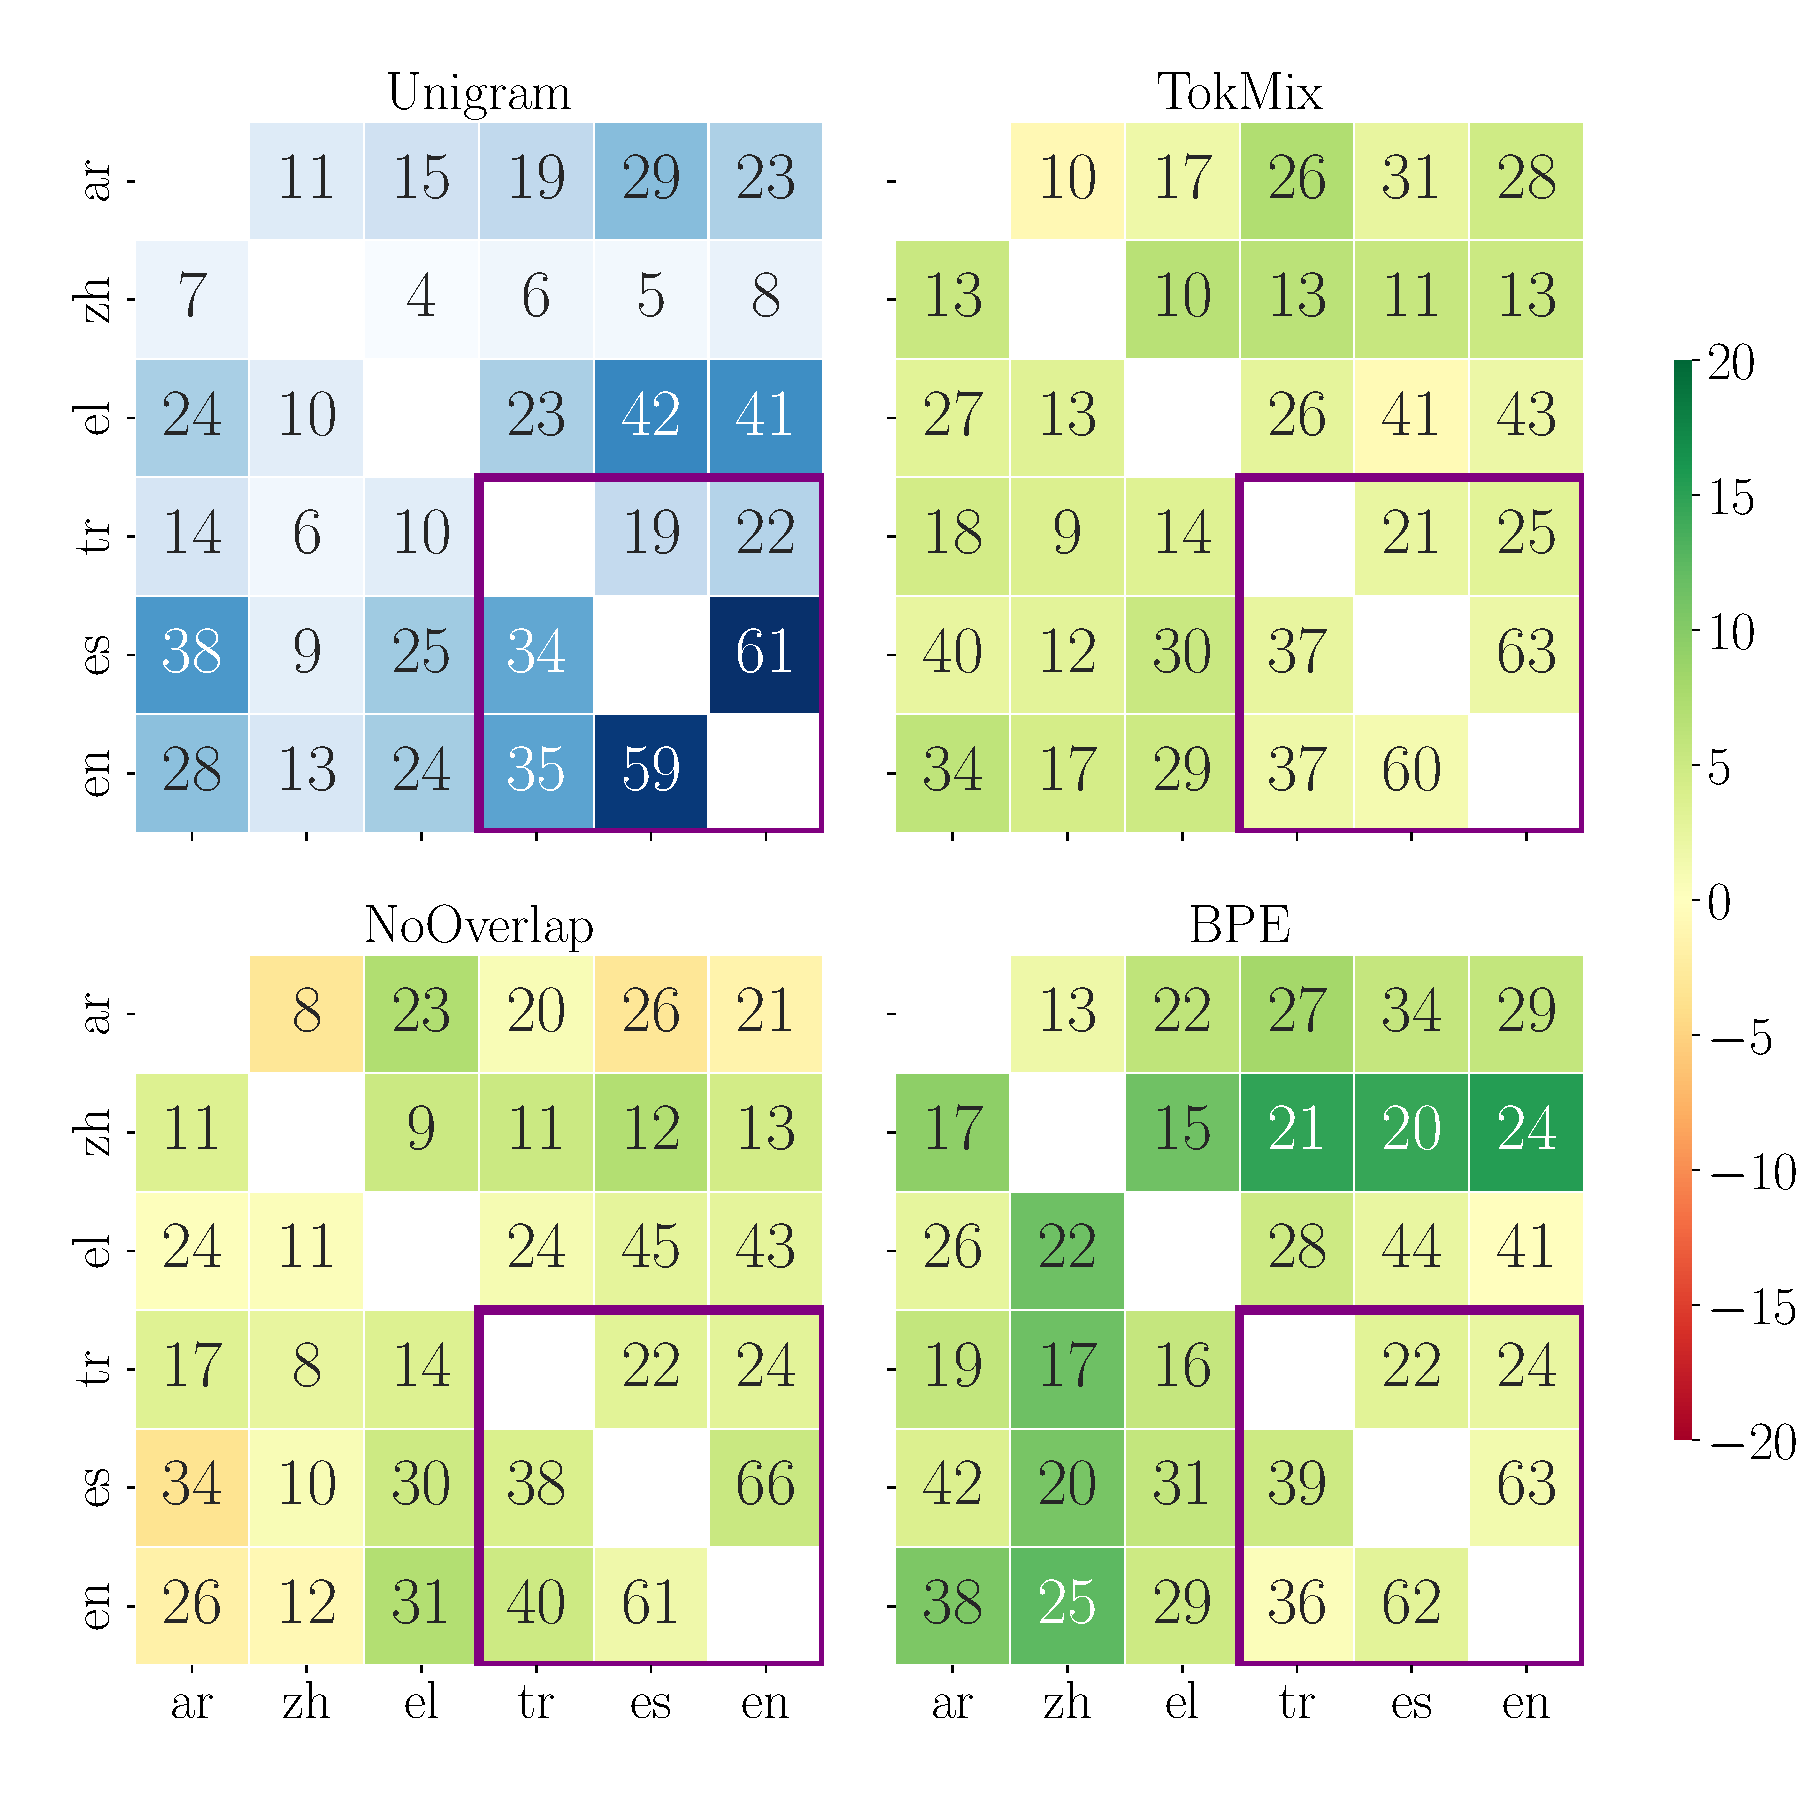
\includegraphics[width=\textwidth]{figures/POS_F1_transfer_.pdf}
        \caption{POS (F1)}
        \label{fig:pos_transfer}
    \end{subfigure}

    \caption{Cross-lingual transfer for POS and NER tasks. The absolute values are presented for the Unigram tokenizer. For other tokenization methods, the color scheme shows a difference from the Unigram algorithm. In the case of NER, we observe a drop in cross-lingual transfer for \textsc{NoOverlap} tokenization, especially for the same script pairs, suggesting that lexical overlap is an important aspect contributing to cross-lingual transfer for NER. We don't see similar drop in the case of Part of Speech tagging.}
\end{figure*}

